\section{method}


%///// Need to combine these two parts into one for data set


\subsection{DataSet}
We use a sample of nearly 150 million geo-tagged, timestamped Flickr
photos as our source of user-contributed observational data about the
world. We collected this data using the public Flickr API, by
repeatedly searching for photos within random time periods and
geo-spatial regions, until the entire globe and all days between January 1, 2007 and December 31, 2010 had been covered.
We applied filters to remove blatantly inaccurate
metadata, in particular removing photos with geotag precision less
than about city-scale (as reported by Flickr), and photos whose upload
timestamp is the same as the EXIF camera timestamp (which usually
means that the camera timestamp was missing).  

For ground truth we use large-scale data originating from two
independent sources: ground-based weather stations, and aerial
observations from satellites.  For the ground-based observations, we
use publicly-available daily snowfall and snow depth observations from
the U.S. National Oceanic and Atmospheric Administration (NOAA) Global
Climate Observing System Surface Network (GSN)~\cite{ghcn}.  This data
provides highly accurate daily data, but only at sites that have
surface observing stations. 
%
For denser, more global coverage, we also use
data from the Moderate Resolution Imaging Spectroradiometer (MODIS)
instrument aboard NASA's Terra satellite. The satellite is in a polar
orbit so that it scans the entire surface of the earth every day. The
MODIS instrument measures spectral emissions at various wavelengths,
and then post-processing uses these measurements to estimate ground cover.
In this paper we use two datasets: the daily snow cover
maps~\cite{modissnow} and the two-week vegetation
averages~\cite{modisveg}. Both of these sets of data including an
estimate of the percentage of snow or vegetation ground cover at each
point on earth, along with a quality score indicating the confidence
in the estimate. Low confidence is caused primarily by cloud cover
(which changes the spectral emissions and prevents accurate ground
cover from being estimated), but also by technical problems with the
satellite. 
As an example, Figure~\ref{fig:samplemap} shows raw satellite snow data from one particular day.


\subsubsection{Snow DataSet}
% Create training data to  build snow visual model

The distribution of geo-tagged Flickr photos is highly
non-uniform, with high peaks in population centers and tourist
locations.  Sampling uniformly at random from  Flickr photos
produces a dataset that mirrors this highly non-uniform distribution,
biasing it towards cities and away from rural areas. Since our
eventual goal is to reproduce continental-scale satellite maps, rural
areas are very important. An alternative is biased sampling that
attempts to select more uniformly over the globe, but has the
disadvantage that it no longer reflects the distribution of Flickr
photos. Other important considerations include how to find a variety
of snowy and non-snowy images, including relatively difficult images
that may include wintry scenes with ice but not snow, and how to
prevent highly-active Flickr users from disproportionately affecting
the datasets.

We strike a compromise on these issues by combining together datasets
sampled in different ways.  We begin with a collection of about 100
million Flickr photos geo-tagged within North America and collected
using the public API (by repeatedly querying at different times and
geo-spatial areas, similar to~\cite{hays}). From this set, we
considered only photos taken before January 1, 2009 (so that we could
use later years for creating a separate test set), and selected:
%
%\begin{enumerate}
%\item
(1) all photos tagged \textit{snow,} \textit{snowfall,} \textit{snowstorm,} or \textit{snowy} in
  English and 10 other common languages (about 500,000 images);
%\item
(2) all photos tagged \textit{winter} in English and about 10 other languages (about 500,000 images);
%\item
(3) a random sample of 500,000 images.
%\end{enumerate}
%
This yielded about 1.4 million images after removing duplicates.  We
further sampled from this set in two ways. First, we selected up to 20
random photos from each user, or all photos if a user had less than 20
photos, giving about 258,000 images. Second, we sampled up to 100
random photos from each $0.1^\circ \times 0.1^\circ$
latitude-longitude bin of the earth (roughly 10km $\times$ 10km at the
mid latitudes), yielding about 300,000 images. The combination of
these two datasets has about 425,000 images after removing duplicates,
creating 
a diverse and realistic selection
of images.  We partitioned this dataset into test and training
sets on a per-user basis, so that all of any given user's photos are
in one set or the other  (to reduce the potential
for duplicate images appearing in both
training and test).

We then presented a subset of these images to humans and collected
annotations for each image. We asked people to label
the images into one of four categories: (1) contains obvious
snow near the camera; (2) contains a trace amount of snow near
the camera; (3) contains obvious snow but far away from the
camera (e.g. on a mountain peak); and (4) does not contain snow. 
For our application of reconstructing snowfall maps, we consider (1)
and (2) to be positive classes and (3) and (4) to be negative,
since snowfall in the distance does not give evidence of snow
at the image's geo-tagged location. In total we labeled 10,000 images.

\subsubsection{Vegetation DataSet}
%%% Need to describe the training data for build vegetation visual model


We build a data set with over 10000 images. They are taken before 2009, and are composed by images with "forest" and "summer" like tags and also random images without any tag preference. These images are labeled with categories 
\textit{"Outdoor Greenery","Outdoor non-Greenery","Indoor","Other-modified"},and \textit{"Not available"}.

Finally, we build a positive set with images in category \textit{"Outdoor Greenery"} and a negative set 
with images in categories \textit{"Outdoor non-Greenery"} and \textit{"Indoor"}. To learn a image classification model, we build a training set with 4000 images and a testing set with 1900 images. In training and testing set, there are equal number of positive and negative samples.
To show the diversity of our Flickr image dataset, in figure ~\ref{fig:dataset} we present a random sample of images in our vegetation dataset labeled as positive and negative.









\begin{figure*}[th]
{\small{
\begin{center}
\begin{tabular}{@{}c@{\,\,\,}c@{\,\,\,}c@{\,\,\,}c@{\,\,\,}c@{\,\,\,}}
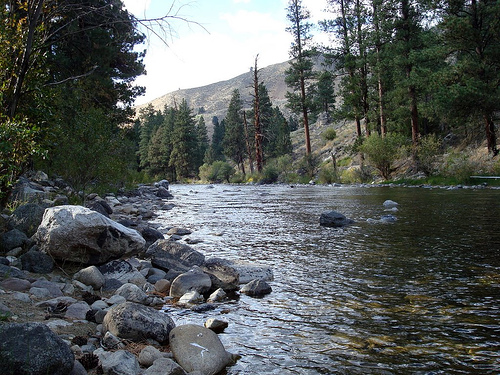
\includegraphics[width=0.19\textwidth]{imggrid/datasetposi/1.jpg} &
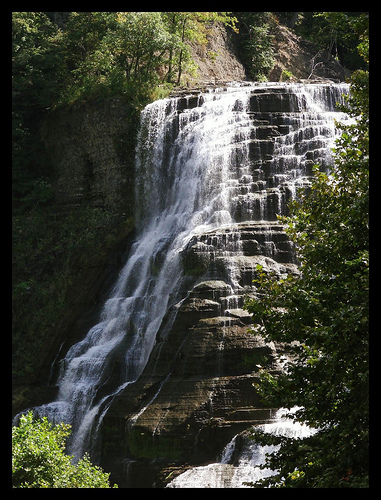
\includegraphics[height=1in]{imggrid/datasetposi/2.jpg} &
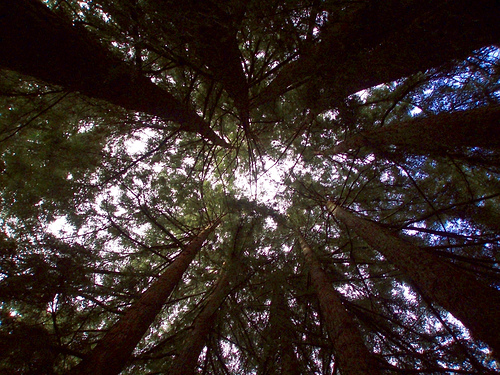
\includegraphics[width=0.19\textwidth]{imggrid/datasetposi/3.jpg} &
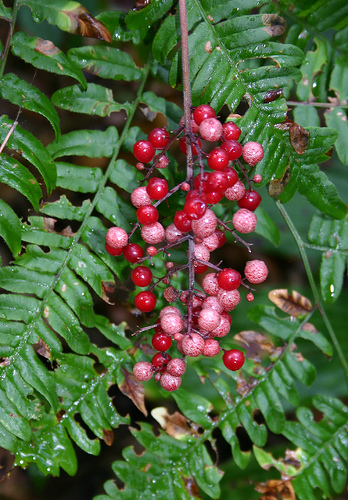
\includegraphics[height=1in]{imggrid/datasetposi/4.jpg} &
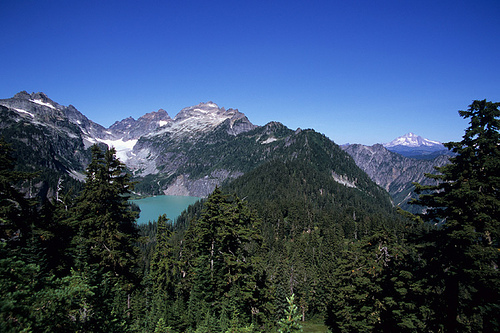
\includegraphics[width=0.19\textwidth]{imggrid/datasetposi/5.jpg} \\
%\multicolumn{5}{c}{(a) Random positive images in vegetation dataset} \\
\\[-6pt]
\hline
\\[-6pt]
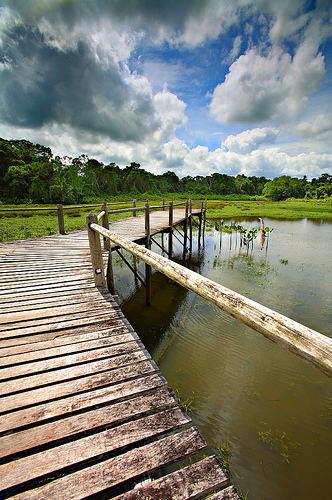
\includegraphics[height=1in]{imggrid/datasetposi/6.jpg} &
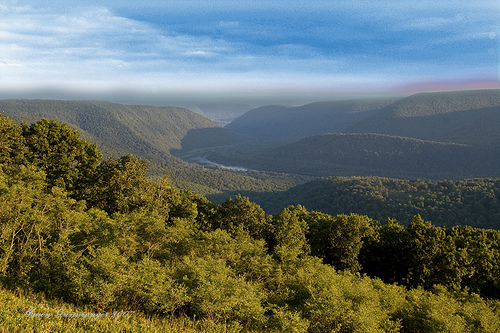
\includegraphics[width=0.19\textwidth]{imggrid/datasetposi/7.jpg} &
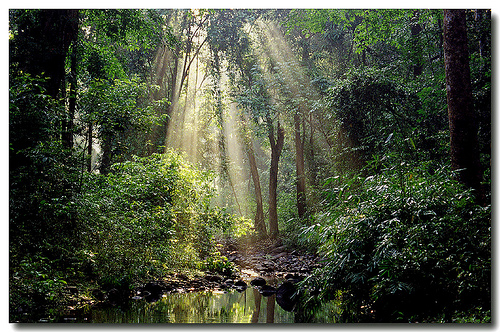
\includegraphics[width=0.19\textwidth]{imggrid/datasetposi/8.jpg} &
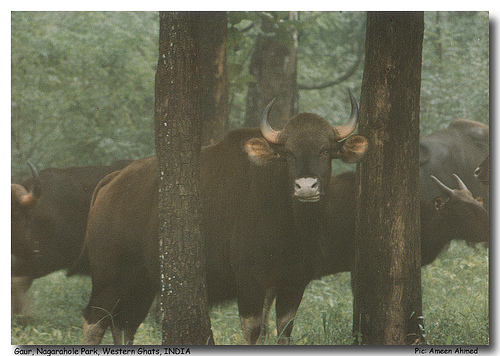
\includegraphics[width=0.19\textwidth]{imggrid/datasetposi/9.jpg} &
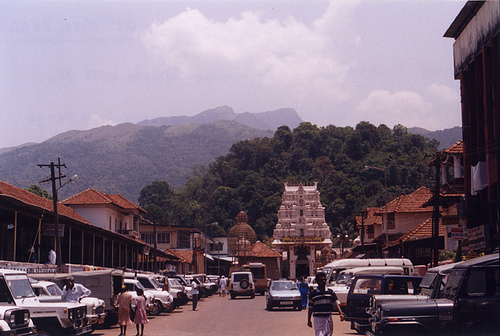
\includegraphics[width=0.19\textwidth]{imggrid/datasetposi/10.jpg} \\
\multicolumn{5}{c}{(a) Random positive images in vegetation dataset} \\ 
\\[-6pt]
\hline
\\[-6pt]
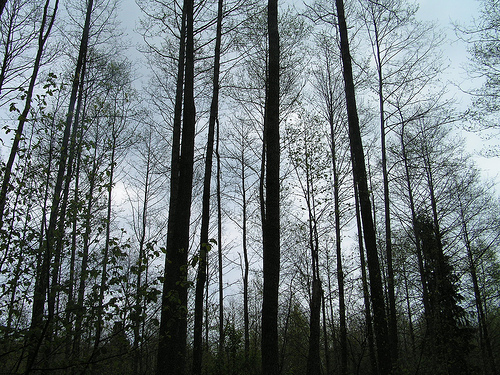
\includegraphics[width=0.19\textwidth]{imggrid/datasetnega/1.jpg} &
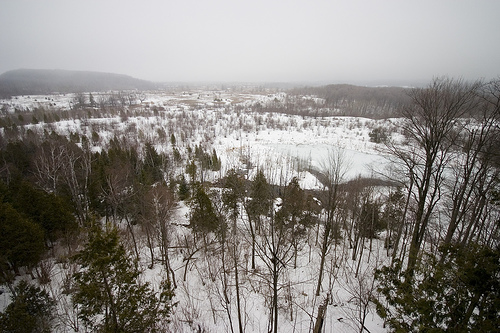
\includegraphics[width=0.19\textwidth]{imggrid/datasetnega/2.jpg} &
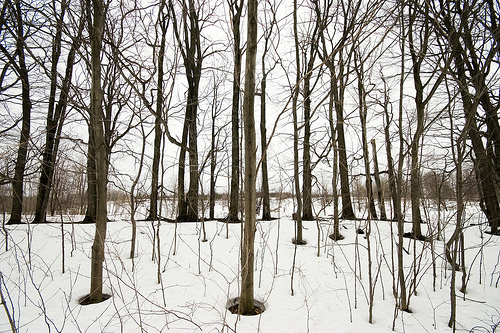
\includegraphics[width=0.19\textwidth]{imggrid/datasetnega/3.jpg} &
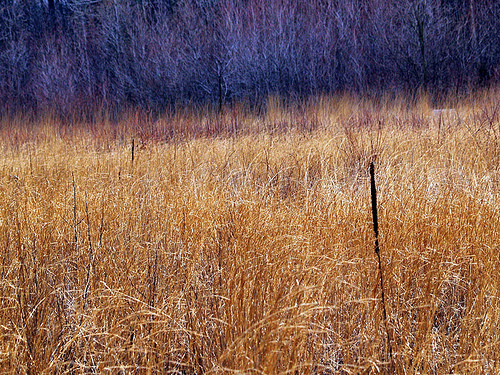
\includegraphics[width=0.19\textwidth]{imggrid/datasetnega/4.jpg} &
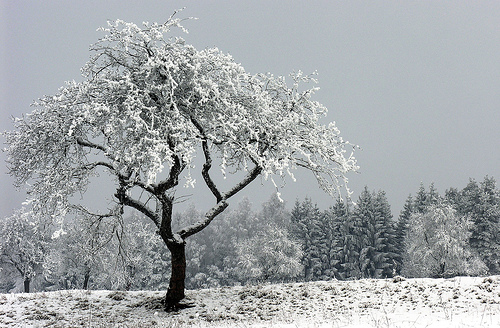
\includegraphics[width=0.19\textwidth]{imggrid/datasetnega/5.jpg} \\
%\multicolumn{5}{c}{(c) Random false negatives (snow images classified as non-snow)} \\ 
\\[-6pt]
\hline
\\[-6pt]
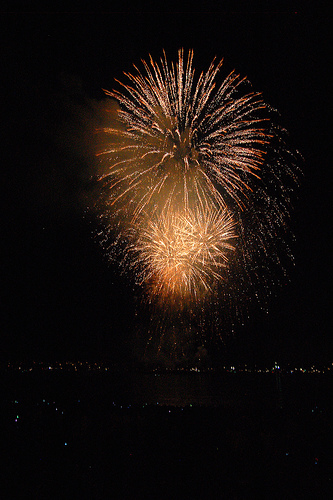
\includegraphics[height=1in]{imggrid/datasetnega/6.jpg} &
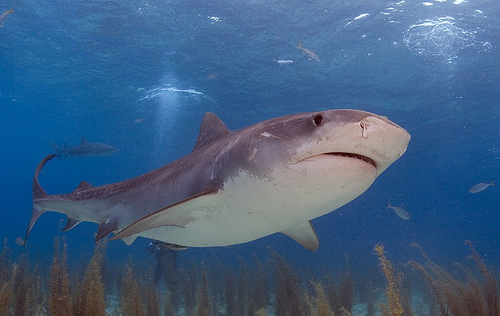
\includegraphics[width=0.19\textwidth]{imggrid/datasetnega/7.jpg} &
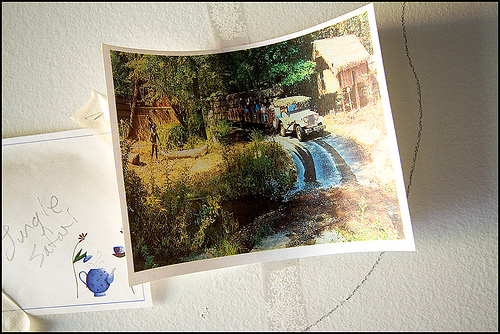
\includegraphics[width=0.19\textwidth]{imggrid/datasetnega/8.jpg} &
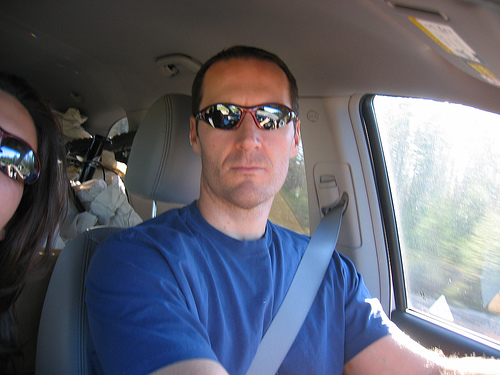
\includegraphics[width=0.19\textwidth]{imggrid/datasetnega/9.jpg} &
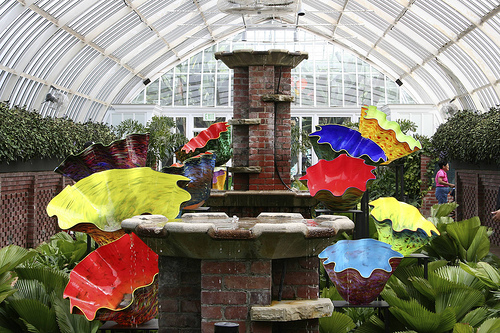
\includegraphics[width=0.19\textwidth]{imggrid/datasetnega/10.jpg} \\
\multicolumn{5}{c}{(b) Random negative images in vegetation dataset} \\
\end{tabular}
\end{center}
}}
\caption{Random images from our hand-labeled dataset. Public sharing images are various in quality, contents, illumination and view angle.
Negative images like winter trees without leaves, or indoor images capturing a photo of forest are more confusing.}
\label{fig:dataset}
\end{figure*}


In continental-scale prediction, we only look at images on Flickr.com in year 2007 to 2010, with no tag limitation. We filter out the photos with inaccurate timestamps and geotags. We only use images with geotag precision no less than 13. ( what's that mean?) 

I paste this from David's email. The only thing is we use geotag precision >= 13 rather than 11. 

[For geotags, there is an
accuracy number right after the GPS coordinate in the merge\_files; we
should ignore any photos with a number less than about 11. That means
that the precision is less than about a city-scale. For timestamps,
one thing that happens a lot is that people upload photos to Flickr
that do not have timestamps -- e.g. scanned images. By default, Flickr
gives this photo a timestamp of the day and time that it was
*uploaded*. The first date in the merge\_files is the taken time and
the second is the upload time. So if these two are the same, it means
the taken time is probably not right and we should ignore the photo.
Now one complication is that the two timestamps are in different time
zones -- taken time is in the user's timezone while upload time is in
Flickr's time zone (pacific time I think). So a simple rule is to
simply remove any photos whose minutes and seconds are exactly the
same for both taken time and upload time. That will unnecessarily
remove about 1/(60*60)=1/3600 photos, but is a good simple rule.]




\subsection{Extracting semantics using tags from individual images}

We consider two learning paradigms. The first
is to produce a single exemplar for each bin in time and space
consisting of the set of all tags used by all users. For each of these
exemplars, the NASA and/or NOAA ground truth data gives a label (snow
or non-snow). We then use standard machine learning algorithms like
Support Vector Machines and decision trees to identify the most
discriminative tags and tag combinations. In the second paradigm, our
goal instead is to classify individual \textit{photos} as containing
snow or not, and then use these classifier outputs to compute the
number of positive and non-positive photos in each bin (i.e., to
compute $m$ and $n$ in the likelihood ratio described in the last
section).

\subsection{Extracting semantics using images from individual images}


%\subsubsection{Traditional Visual features}

\subsubsection{Snow Visual features}
Snow is a somewhat unique visual phenomenon, and we claim that
detecting it in images is a unique recognition task. In some cases,
snow can be detected by coarse scene recognition: ski slopes or snowy
landscapes are distinctive scenes. But snow can appear in any kind of
outdoor scene, and is thus like an object. However, unlike most
objects that have some distinctive features, snow is simply a white,
near-textureless material.  (In fact, our informal observation is that
humans detect snow not by recognizing its appearance, but by noticing
that other expected features of a scene are occluded; in this sense,
detecting snow is less about the features that are seen and more about
the features that are \textit{not} seen. We leave this as an
observation to inspire future work.)
%
We tested a variety of off-the-shelf visual features for classifying
whether an image contains fallen snow. We used Support Vector
Machines for classification, choosing kernels based on the feature
type.  Intuitively, color is a very important feature for detecting
snow, and thus we focused on features that use color to some
degree. Our features are:


\xhdr{Color histograms} We begin with perhaps the simplest of color
features. We build joint histograms in CIELAB space, with 4 bins on
the lightness dimension and 14 bins along each of the two color
dimensions, for a total of 784 bins. We experimented with other
quantizations and found that this arrangement worked best.  We encode
the histogram as a 784 dimensional feature and use an SVM with a
chi-squared distance (as in~\cite{XiaoHEOT10}).

\xhdr{Tiny images} 
%Tiny images are another very simple way of
%representing an image that nevertheless capture coarse color and
%spatial layout information
We subsample images to 16 $\times$ 16 pixels, giving 256 pixels per
RGB color plane and yielding a 768 dimensional feature vector.
Drastically reducing the image dimensions yields a feature that is
less sensitive to exact alignment and more computationally
feasible~\cite{torralba2008tiny}.  
%We use an RBF kernel to compare the
%unnormalized distance.


\xhdr{Spatial Moments} Tiny images capture coarse color and spatial
scene layout information, but much information is discarded during
subsampling.  As an alternative approach, we convert the image to LUV
color space, divide it into 49 blocks using a 7 $\times$ 7 grid, and
then compute the mean and variance of each block in each color
channel.  Intuitively, this is a low-resolution image and a very
simple texture feature, respectively.  We also compute maximum,
minimum, and median value within each cell, so that the final
feature vector has 735 dimensions.

%<<<<<<< .mine

%\begin{figure*}[th!]
%\begin{center}
%\vspace{-16pt}
%\begin{tabular}{cc}
% 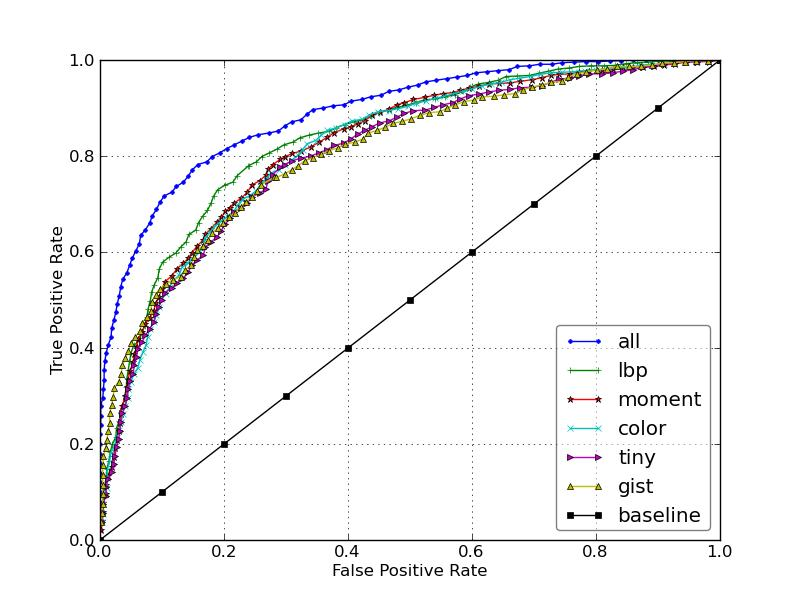
\includegraphics[width=0.4\textwidth]{figs/ROC-curves.jpg} &
%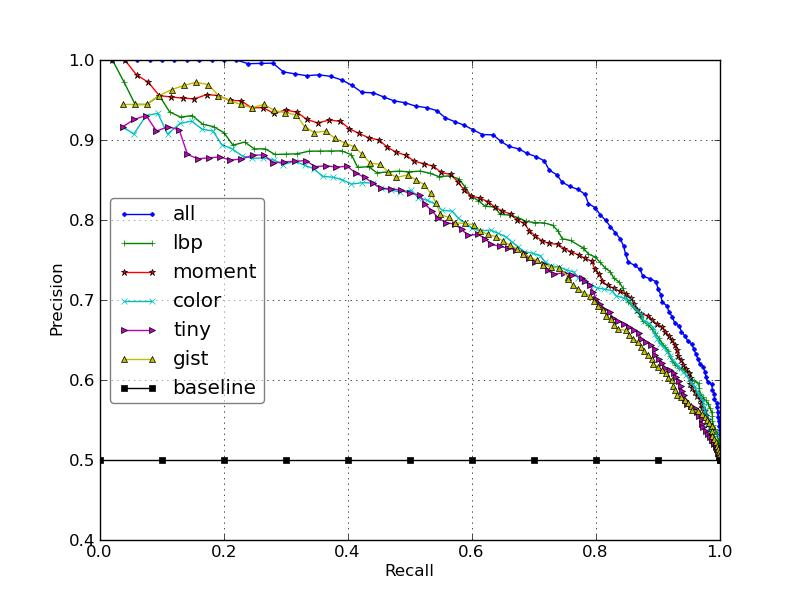
\includegraphics[width=0.4\textwidth]{figs/PR-curves.jpg} \\
%\end{tabular}
%\end{center}
%\vspace{-12pt}
%\caption{
%Snow classification results for different features and combinations, in terms of {\textit{(left):}} ROC curves for the task of classifying snow vs. non-snow images; and 
%{\textit{(right):}} Precision-Recall curves for the task of retrieving snow images.
%}
%\label{fig:PR_ROC_snow}
%\end{figure*}


\xhdr{{Color Local Binary Pattern (LBP) with pyramid
    pooling}} LBP represents each $9 \times 9$ pixel neighborhood 
as an 8-bit binary number by thresholding the 8 outer pixels
by the value at the center.  We build 256-bin histograms over
these LBP values, both on the grayscale image and on each RGB color
channel~\cite{korayem2012solving}. We compute these histograms in each cell of a three-level spatial
pyramid, with 1 bin at the lowest level, 4 bins in a $2 \times 2$ grid
at the second level, and 16 bins in a $4 \times 4$ grid at the third level.
This yields a $(1+4+16) \times 4 \times 256$ = 21504 dimensional feature
vector for each image.

\xhdr{GIST} We also apply GIST features, which capture coarse texture
and scene layout by applying a Gabor filter bank followed by
down-sampling~\cite{oliva2001modeling}. Our variant produces a
1536-dimensional  vector and operates on color planes. Scaling
images to have square aspect ratios before computing GIST improved
classification results significantly~\cite{douze2009evaluation}.


We experimented with a number of other features, and found
that they did not work well; local features like SIFT and HOG in
particular perform poorly, again because snow does not have
distinctive local visual appearance. 

\subsubsection{Vegetation visual features}

Vegetation has the signature green color. 
The leaves of plants have distinctive visual texture. 
So we employ SIFT feature to analyze the local gradient distribution. 
And we also extract GIST feature to describe texture feature and global context. 





\textbf{\textit{Color SIFT histogram.}}
We extract dense SIFT feature on each of the RGB color plane, and concatenate them to build color SIFT feature. The dense SIFT feature is extracted from every 2 pixels by 2 pixels bin, with a step size of 5 pixels. In this way, we achieve representative key points and reasonable computation complex. 
% Therefore we have 128*3-d for each key point
% about 300-500 key points each images

From training data set, We build 2000 dimensional centers of color SIFT feature using K-means clustering. With these centers, a 2000 dimensional histogram is built from all the key points of each image.

Using SIFT histogram, a model is trained and tested with SVM using RBF kernel. 
%Maybe the numbers should be in evaluation section        
%The performance is 78.10\%.

\textbf{\textit{Color GIST.}}
Similar to color SIFT feature, we also extract GIST feature from each of the RGB color plane.\\*\\*
%The performance is 82.58\%.

\textbf{\textit{Combine visual features.}}
The combined visual feature is built from concatenating the normalized GIST feature and SIFT histogram. A new model is learnt based on the combined feature.
%The performance is 85.9\%.

\subsubsection{Deep learning}
Recently the Conventional Neural Network (CNN) ~\cite{krizhevsky2012imagenet} has gained a lot of attention in the vision community, as it outperformed all other techniques in the ImageNet challenge (the most famous object category detection competition)~\cite{ilsvrcarxiv14}.



CNN is a special type of feed forward neural network inspired by the biological process~\cite{krizhevsky2012imagenet} in cats' visual cortex. 
%It is currently the de facto algorithm of image classification on standard datasets.
CNN enjoys additional features that distinguish it from the standard neural networks: shared wights and sparse connectivity.
A layer in CNN may consist of three different stages: convolution, non-linear activation, and pooling.
In the convolution stage, a set of convolution filters is applied in parallel. 
The output of a convolution filter is then passed to non-linear activation functions (e.g., rectified linear activation function, sigmoid activation function).
The final stage is pooling, where the net output is manipulated based on its neighbors (e.g., max pooling , $L_2$ norm, and weighted average).
Pooling makes the network invariant to the translation of the input

The key idea behind this approach is that instead of first designing low-level features by
hand and then running a machine learning algorithm, a single unified
algorithm should learn both the low-level features and the
high-classifier simultaneously. 

We apply CNN to detect snow and vegetation on image level. We followed Oquab~\cite{Oquab14} et al. and started with a model pre-trained on the huge ImageNet dataset then we train our models using hand-labeled data sets.
 



\subsection{Combining evidence together across users}

Our goal is to estimate the presence or absence of a given ecological
phenomenon (like a species of plant or flower, or a meteorological
feature like snow) on a given day and at a given place,
using only the geo-tagged, time-stamped photos from Flickr. One way of viewing
this problem is that every time a user takes a photo of a phenomenon
of interest, they are casting a ``vote''  that the
phenomenon actually occurred in a given geospatial region. 
 We could
simply look for tags indicating the presence of a feature --
i.e. count the number of photos with the tag ``snow'' --  
but sources of noise and bias make this task 
challenging, including:
\begin{packed_itemize}
\item[---] \textit{Sparse sampling:} The geospatial distribution of photos
  is highly non-uniform. A lack of photos
  of a phenomenon in a region does not
  necessarily mean that it was not there. 
\item[---] \textit{Observer bias:} Social media users are younger and
  wealthier than average, and most live in North
  America and Europe.
\item[---] \textit{Incorrect, incomplete and misleading tags:}
  Photographers may use incorrect or ambiguous tags  ---
  e.g. the tag ``snow'' may refer to a snowy owl or interference on a
  TV screen.
\item[---] \textit{Measurement errors:} Geo-tags and timestamps are
  often incorrect (e.g. because people   forget to set their camera clocks).
\end{packed_itemize}

\xhdr{A statistical test.}  We introduce a simple probabilistic model
and use it to derive a statistical test that can deal with some such
sources of noise and bias. The test could be used for estimating the
presence of any phenomenon of interest; without loss of generality we
use the particular case of snow here, for ease of explanation.  Any
given photo either contains evidence of snow (event $s$) or does not
contain evidence of snow (event $\bar{s}$).  We assume that a given
photo taken at a time and place with snow has a fixed probability $P(s
| snow)$ of containing evidence of snow; this probability is less than
1.0 because many photos are taken indoors, and outdoor photos might be
composed in such a way that no snow is visible. We also assume that
photos taken at a time and place without snow have some non-zero
probability $P(s | \overline{snow})$ of containing evidence of snow;
this incorporates various scenarios including incorrect timestamps or
geo-tags and misleading visual evidence (e.g.  man-made
snow).

Let $m$ be the number of snow
photos (event $s$), and $n$ be the number of non-snow photos (event
$\bar{s}$) taken at a place and time of interest. Assuming that each photo is captured
independently, we can use Bayes' Law to
derive the probability that a given place has snow
given its number of snow and non-snow photos,
%
%\newcommand{\smsn}{\overbrace{s\cdots s}^{m},\overbrace{\overline{s}\cdots \overline{s}}^{n}}
%%hp cr: \bar{s}^n
\newcommand{\smsn}{s^m, \bar{s}^n}
\newcommand{\smsntwo}{s^m, \bar{s}^n}
%%\newcommand{\smsn}{s^m, s^n}
%%\newcommand{\smsntwo}{s^m, s^n}
%\newcommand{\smsntwo}{\underbrace{s\cdots s}_{m},\underbrace{\overline{s}\cdots \overline{s}}_{n}}
\begin{eqnarray*}
P(snow|\smsn)  &=&\frac{ P(\smsn|snow)P(snow)}{P(\smsntwo)}  \\
&=&\frac{{m+n\choose m}p^{m}(1-p)^{n}P(snow)}{P(\smsntwo)},  
\end{eqnarray*}
%
where we write $s^m, \bar{s}^n$ to denote $m$ occurrences of event $s$ and $n$ occurrences of event $\bar{s}$, and where $p=P(s|snow)$ and $P(snow)$ is the prior probability of snow. A similar derivation gives the posterior probability that the bin does not contain snow,
%
\begin{eqnarray*}
P(\overline{snow}|\smsn)  &=&\frac{{m+n\choose m}q^{m}(1-q)^{n}P(\overline{snow})}{P(\smsntwo)},  
\end{eqnarray*}
%
where $q=P(s|\overline{snow})$. 
%
Taking the ratio between these two posterior probabilities yields a likelihood ratio,
%
\begin{eqnarray}
\frac{P(snow|\smsn)}{P(\overline{snow}|\smsntwo)}
%\\=\frac{\frac{{m+n\choose m}p^{m}(1-p)^{n}P(snow)}{P(\overbrace{s\cdots s}^{m},\overbrace{\overline{s}\cdots \overline{s}}^{n})}}{\frac{{m+n\choose m}q^{m}(1-q)^{n}P(\overline{snow})}{P(\overbrace{s\cdots s}^{m},\overbrace{\overline{s}\cdots \overline{s}}^{n})}}
&=&\frac{P(snow)}{P(\overline{snow})}\left(\frac{p}{q}\right)^{m}\left(\frac{1-p}{1-q}\right)^n.
\label{eq:conf}
\end{eqnarray}
%
This ratio can be thought of as a measure of the confidence that a
given time and place actually had snow, given photos from Flickr.

A simple way of classifying a photo into a positive event $s$ or a
negative event $\bar{s}$ is to use text tags. We identify a
set ${\cal S}$ of tags related to a phenomenon of
interest. Any photo tagged with at least one tag in ${\cal S}$ is
declared to be a positive event $s$, and otherwise it is considered a
negative event $\bar{s}$. For the snow detection task, we use the set
${\cal S}$=\{snow, snowy, snowing, snowstorm\}, which we selected
by hand.

%%, which we chose by
%%looking at the 200 most frequent Flickr tags and hand selecting those
%%directly relevant to snowfall.

The above derivation assumes that photos are taken independently of
one another, which is generally not true in reality. One particular
source of dependency is that photos from the same user are highly
correlated with one another.  To mitigate this problem, instead of
counting $m$ and $n$ as numbers of \textit{photos}, we instead let $m$ be 
the number of \textit{photographers} having at least one photo with evidence of snow,
while $n$ is the numbers of photographers who did not upload any
photos with evidence of snow.

The probability parameters in the likelihood ratio of
equation~(\ref{eq:conf}) can be directly estimated from training data
and ground truth. For example, for the snow cover results
presented in Section~\ref{sec:results}, the learned parameters are: $p
= p(s|snow) = 17.12\%$, $q = p(s|\overline{snow}) = 0.14\%$.  In other
words, almost 1 of 5 people at a snowy place take a photo containing
snow, whereas about 1 in 700 people take a photo containing evidence
of snow at a non-snowy place.

Figure~\ref{fig:samplemap} shows a visualization of the likelihood
ratio values for the U.S. on one particular day using this simple
technique with ${\cal S}$=\{snow, snowy, snowing, snowstorm\}.  High
likelihood ratio values are plotted
in green, indicating a high confidence of snow in a geospatial bin,
while low values are shown in blue and indicate high confidence of 
no snow.  Black areas indicate a likelihood ratio 
near 1, showing little conference either way, and grey areas lack
data entirely (having no Flickr photos in that bin on that day).



%\xhdr{Temporal smoothing.}  For many phenomena (including snow), the
%existence of an event on one day is strongly correlated with its
%existence on the next day. Thus one way of addressing the sparsity of
%Flickr photos in some locations is to propagate evidence forward and
%backward in time.  To do this, we apply a Gaussian filter on the Flickr
%confidence values for each bin in an attempt to achieve better
%recalls. We vary the degree of smoothing by using Gaussians with
%different variance values.  We tried smoothing with many
%different parameters, including smoothing both forward and backwards
%in time, or in only one direction.

% I really suggest we take this off. Not get any help from time and location data, and not do any 
%post-process to is a selling point of our paper. And we are not doing this after WWW paper
%any more.


\xhdr{Voting.}  Voting is an interesting
technique  because of its simplicity. Voting
simply counts the number of users who have annotated at least one
photo in a given bin and day with a snow-related tag.
Figure~\ref{fig:precvotes}
plots precision versus the number of votes for snow retrieval.  The
shape of these curve illustrates why crowd-sourced observations of the
world can be reliable, if enough people are involved: as the number of
votes for snow increases, it becomes progressively less likely that
these independent observations are coincidental, and more likely that
they are caused by the presence or absence of an actual phenomenon.
It is interesting to notice that when there are 7 or more snow voters,
snow prediction precision becomes 100\%, while the same is true for
non-snow prediction when the number of non-snow voters reaches 33
if there are no snow voters in the bin.

\begin{figure}
\begin{center}
\begin{tabular}{c}
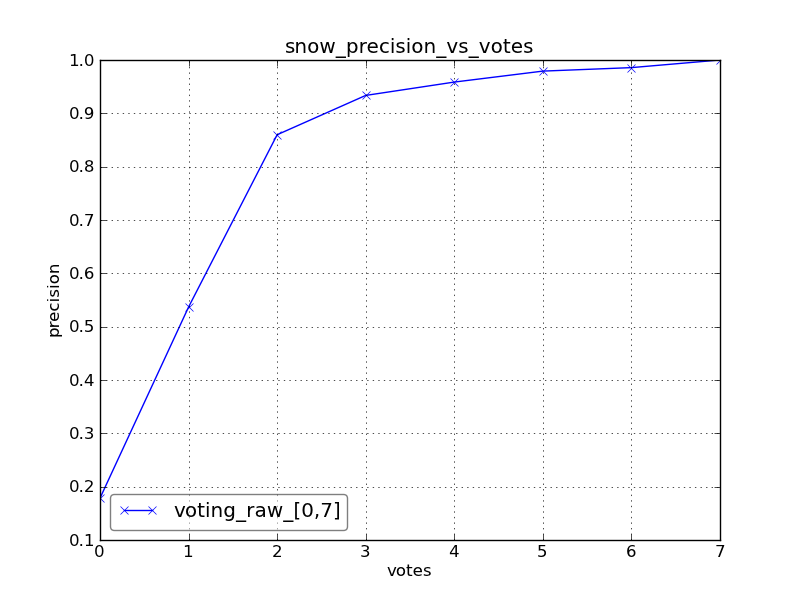
\includegraphics[width=0.3\textwidth,trim=1cm 0.5cm 1cm 1cm,clip]{plots/precvotes.png}
%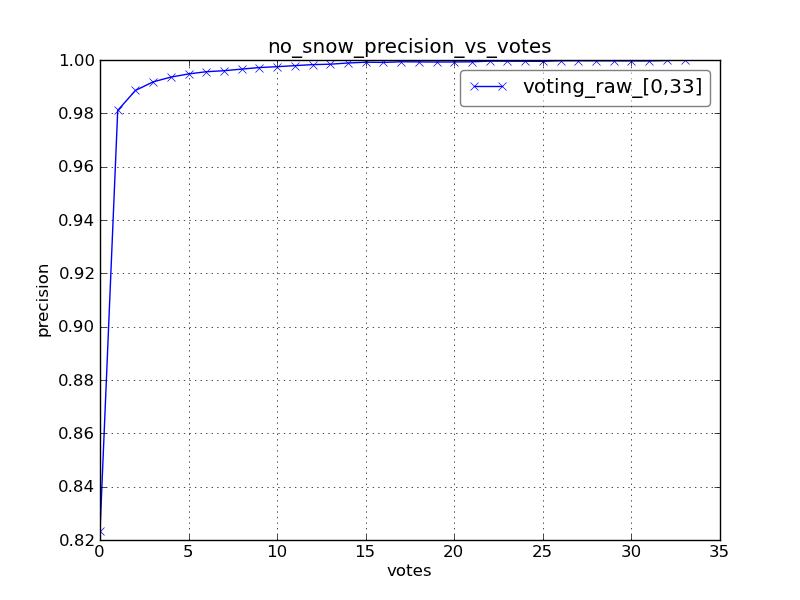
\includegraphics[width=0.3\textwidth,trim=1cm 1cm 1cm 1cm,clip]{plots/precvotesnosnow.png} \\
\end{tabular}
\end{center}
\vspace{-20pt}
\caption{Precision vs number of votes for snow predictions using the voting method.}
\label{fig:precvotes}
\end{figure}
%\hfill \break
%\hfill \break
%\subsection*{latest writing}
%\hfill \break
%\hfill \break


%Three parts:
%
%A. Extracting semantics using tags from individual images, which is what we did in WWW paper. Discuss simple keyword search on e.g. a few snow words, or machine learning to find keyword combinations. 
%
%B. Extracting semantics using images from individual images. Here we talk about the traditional features that are covered in ICCV paper, and then the deep learning techniques.
%
%C. Combining evidence together across users. **Here we have the simple voting method and the probabilistic confidence score. We can augment with the additional factors that Stefan suggested, including priors based on time of year or geographic location, or other evidence like historical accuracy of specific users.] Also including temporal and spatial smoothing by simply adding to the confidence score priors.
%
%[Note what I am omitting here. My preference would be to ignore any techniques that try to classify bins jointly by aggregating all the tags or visual features of photos together in a bin and then using those features. I would also really like if the final classification is based just on thresholding a confidence score, even if the results are slightly worse than the best we can do. I just think it makes the story more complicated to do otherwise and harder to justify.] 
%
%\hfill \break
%\hfill \break
%===================================
%\hfill \break
%\hfill \break






\begin{comment}

%\subsection{Datasets}
\begin{comment}
We use a sample of nearly 150 million geo-tagged, timestamped Flickr
photos as our source of user-contributed observational data about the
world. We collected this data using the public Flickr API, by
repeatedly searching for photos within random time periods and
geo-spatial regions, until the entire globe and all days between January 1, 2007 and December 31, 2010 had been covered.
We applied filters to remove blatantly inaccurate
metadata, in particular removing photos with geotag precision less
than about city-scale (as reported by Flickr), and photos whose upload
timestamp is the same as the EXIF camera timestamp (which usually
means that the camera timestamp was missing).  

For ground truth we use large-scale data originating from two
independent sources: ground-based weather stations, and aerial
observations from satellites.  For the ground-based observations, we
use publicly-available daily snowfall and snow depth observations from
the U.S. National Oceanic and Atmospheric Administration (NOAA) Global
Climate Observing System Surface Network (GSN)~\cite{ghcn}.  This data
provides highly accurate daily data, but only at sites that have
surface observing stations. 
%
For denser, more global coverage, we also use
data from the Moderate Resolution Imaging Spectroradiometer (MODIS)
instrument aboard NASA's Terra satellite. The satellite is in a polar
orbit so that it scans the entire surface of the earth every day. The
MODIS instrument measures spectral emissions at various wavelengths,
and then post-processing uses these measurements to estimate ground cover.
In this paper we use two datasets: the daily snow cover
maps~\cite{modissnow} and the two-week vegetation
averages~\cite{modisveg}. Both of these sets of data including an
estimate of the percentage of snow or vegetation ground cover at each
point on earth, along with a quality score indicating the confidence
in the estimate. Low confidence is caused primarily by cloud cover
(which changes the spectral emissions and prevents accurate ground
cover from being estimated), but also by technical problems with the
satellite. 
As an example, Figure~\ref{fig:samplemap} shows raw satellite snow data from one particular day.

\end{comment}


%% \begin{figure}
%% \begin{center}
%% \begin{tabular}{cc}
%% 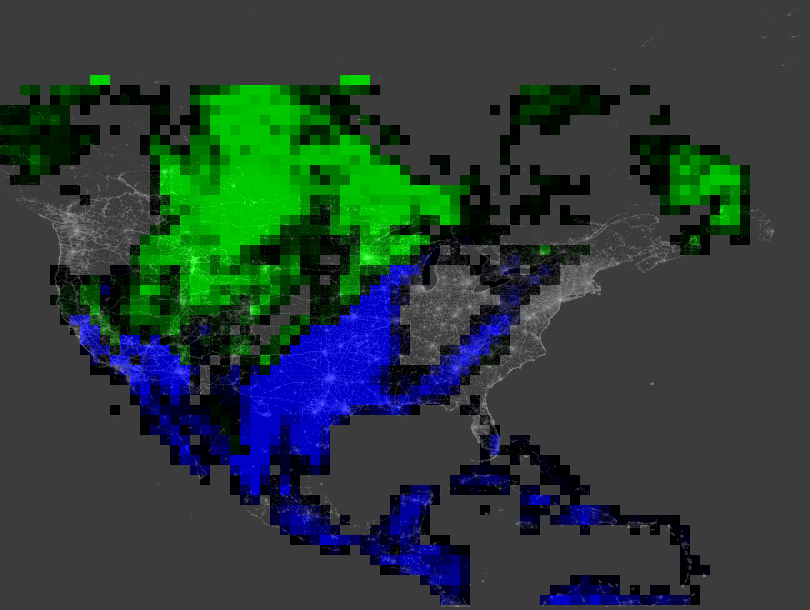
\includegraphics[width=0.5\textwidth]{plots/nasadownsample20070101.png}
%% \end{tabular}
%% \end{center}
%% \caption{Down-sampled NASA MODIS snow coverage data for North America
%%   on 2007.01.01. Grey: water-covered, or no data, or the confidence
%%   index value is 0; blue: no snow and has non-zero confidence index
%%   value; green: has snow and non-zero confidence index value. (Please
%%   view in color.)}
%% \label{fig:nasadownsample20070101}
%% \end{figure}




